\documentclass{beamer}

\usepackage[slovene]{babel}
\usepackage{amsfonts,amssymb}
\usepackage[utf8]{inputenc}
\usepackage{lmodern}
\usepackage[T1]{fontenc}

\usetheme{Warsaw}

\newtheorem{izrek}{Izrek}
\newtheorem{definicija}{Definicija}
\newtheorem{primer}{Primer}
\newtheorem{trditev}{Trditev}
\newtheorem{lema}{Lema}
\newtheorem{oznaka}{Oznaka}

\newcommand{\pojem}[1]{\textsc{#1}}

\DeclareMathOperator{\re}{Re}


\title{Fareyevo zaporedje in Riemannova hipoteza}
\author{Tjaša Vrhovnik}

\institute{Mentor: izr.~prof.~dr.~Aleš Vavpetič\\
	Univerza v Ljubljani\\
	Fakulteta za matematiko in fiziko\\
	Oddelek za matematiko}
\date{13.\ september 2019}

\begin{document}

%%%%%%%%%%%%%%%%%%%%%%%%%%%%%%%%%%%%%%%%%%%

\begin{frame}
\titlepage
\end{frame}

%%%%%%%%%%%%%%%%%%%%%%%%%%%%%%%%%%%%%%%%%%%

\begin{frame}
\frametitle{Struktura diplomskega dela}

\begin{enumerate}
\item Fareyevo zaporedje: motivacija, definicija, lastnosti, dolžina zaporedja
\item Fordovi krogi: lastnosti, posplošitev, Fordove krogle, M\"obiusove transformacije na množici Fordovih krogov
\item Riemannova hipoteza: ekvivalentni trditvi, povezava hipoteze s Fareyevim zaporedjem
\end{enumerate}

\end{frame}

%%%%%%%%%%%%%%%%%%%%%%%%%%%%%%%%%%%%%%%%%%%

\begin{frame}
\frametitle{Fareyevo zaporedje}

\pause
\begin{definicija}
\label{def:Farey}
\emph{Fareyevo zaporedje reda n} oz.\ \emph{n-to Fareyevo zaporedje} je množica racionalnih števil $\frac{p}{q}$ urejenih po velikosti, kjer sta $p$ in $q$ tuji si števili, ter velja $0 \leq p \leq q \leq n$. Označimo ga z $F_n$.

Ekvivalentno, $F_n$ vsebuje vse okrajšane ulomke med $0$ in $1$ z imenovalci, kvečjemu enakimi $n$.
\end{definicija}

\begin{primer}
\(F_1 = \left \{\frac{0}{1}, \frac{1}{1} \right \}, \)

\(F_2 = \left \{\frac{0}{1}, \frac{1}{2}, \frac{1}{1} \right \}, \)

\(F_3 = \left \{\frac{0}{1}, \frac{1}{3}, \frac{1}{2}, \frac{2}{3}, \frac{1}{1} \right \}, \)

\(F_4 = \left \{\frac{0}{1}, \frac{1}{4}, \frac{1}{3}, \frac{1}{2}, \frac{2}{3}, \frac{3}{4}, \frac{1}{1} \right \}. \)
\end{primer}

\end{frame}

%%%%%%%%%%%%%%%%%%%%%%%%%%%%%%%%%%%%%%%%%%%

\begin{frame}
\frametitle{Fareyevo zaporedje}

\begin{definicija}
Sosednja člena v Fareyevem zaporedju imenujemo \emph{Fareyeva soseda}.
\end{definicija}

\begin{definicija}
Naj bosta $\frac{a}{b}$ in $\frac{c}{d}$ sosednja člena nekega Fareyevega zaporedja. Ulomek \[\frac{a+c}{b+d} \] imenujemo \emph{medianta}.
\end{definicija}

\pause
\begin{lema}
\label{lema:EltVišReda}
Dano naj bo Fareyevo zaporedje. Elemente zaporedja višjega reda dobimo z računanjem mediant elementov danega zaporedja.
\end{lema}

\end{frame}

%%%%%%%%%%%%%%%%%%%%%%%%%%%%%%%%%%%%%%%%%%%

\begin{frame}
\frametitle{Fareyevo zaporedje}

\begin{trditev}[Lastnost Fareyevih sosedov]
Naj velja \( 0 \leq \frac{a}{b} < \frac{c}{d} \leq 1\). Ulomka $\frac{a}{b}$ in $\frac{c}{d}$ sta Fareyeva soseda v nekem Fareyevem zaporedju natanko tedaj, ko velja \(bc - ad = 1\).
\end{trditev}

\pause
\begin{block}{Lastnost mediante}
Medianta $\frac{a+c}{b+d}$ je enolično določena z ulomkoma $\frac{a}{b}$ in $\frac{c}{d}$.
\end{block}

\end{frame}

%%%%%%%%%%%%%%%%%%%%%%%%%%%%%%%%%%%%%%%%%%%

\begin{frame}
\frametitle{Fareyevo zaporedje}

\begin{trditev}
\label{trd:DolzinaZap}
Naj bo $\varphi$ Eulerjeva funkcija. Dolžina Fareyevega zaporedja reda n je enaka
\begin{equation}
|F_{n}| = |F_{n-1}| + \varphi(n).
\end{equation}
\end{trditev}

\begin{trditev}
\label{trd:AsimptotDolzina}
Asimptotično se dolžina Fareyevega zaporedja obnaša kot
\begin{equation}
|F_{n}|\sim\frac{3n^2}{\pi^2}.
\end{equation}
\end{trditev}

\end{frame}

%%%%%%%%%%%%%%%%%%%%%%%%%%%%%%%%%%%%%%%%%%%%

\begin{frame}
\frametitle{Fordovi krogi}

\pause
\begin{definicija}
Naj bosta $p$ in $q$ tuji si števili v množici celih števil.
\emph{Fordov krog} C($\frac{p}{q}$) je krog v zgornji polravnini, ki se abscisne osi dotika v točki $\frac{p}{q}$, njegov polmer pa meri $\frac{1}{2q^2}$. 
\end{definicija}

\begin{figure}[h!]
\begin{center}
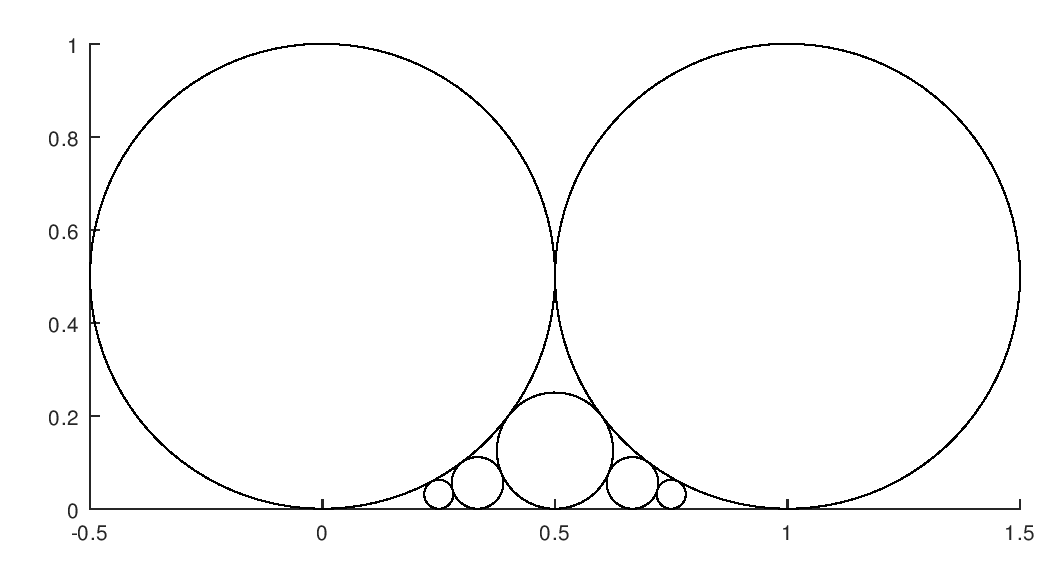
\includegraphics[scale=0.4]{fordovi_krogi.png}
\caption{Fordovi krogi na intervalu $[0,1]$ s polmeri $\protect{\frac{1}{2}}$, $\protect{\frac{1}{8}}$, $\protect{\frac{1}{18}}$ in $\protect{\frac{1}{32}}$.}
\end{center}
\end{figure}

\end{frame}

%%%%%%%%%%%%%%%%%%%%%%%%%%%%%%%%%%%%%%%%%%%%

\begin{frame}
\frametitle{Fordovi krogi}

\begin{trditev}
\label{trd:FordDisjTang}
Fordova kroga, ki pripadata različnima okrajšanima ulomkoma, sta bodisi tangentna bodisi disjunktna.
\end{trditev}

\begin{definicija}
Tangentna Fordova kroga imenujemo \emph{Fordova soseda}.
\end{definicija}

\end{frame}

%%%%%%%%%%%%%%%%%%%%%%%%%%%%%%%%%%%%%%%%%%%%

\begin{frame}
\frametitle{Fordovi krogi}

\begin{trditev}[Lastnost Fordovih sosedov]
\label{trd:FordTangentnost}
Fordova kroga C($\frac{a}{b}$) in C($\frac{c}{d}$) sta tangentna natanko tedaj, ko velja \( |bc-ad|=1. \)
\end{trditev}

\begin{trditev}[Lastnost mediante za Fordove kroge]
Naj bosta C($\frac{a}{b}$) in C($\frac{c}{d}$) Fordova soseda. Tedaj obstaja enolično določen Fordov krog C($\frac{a+c}{b+d}$) in je tangenten na izbrana kroga. Imenujemo ga \emph{medianta Fordovih krogov}.
\end{trditev}

\pause
\begin{izrek}
Naj bosta kroga C($\frac{p}{q}$) in C($\frac{P}{Q}$) Fordova soseda. Vse Fordove sosede Fordovega kroga C($\frac{p}{q}$) lahko zapišemo v obliki C($\frac{P_n}{Q_n}$), kjer je $\frac{P_n}{Q_n} = \frac{P+np}{Q+nq}$ in $n$ preteče vsa cela števila.
\end{izrek}

\end{frame}

%%%%%%%%%%%%%%%%%%%%%%%%%%%%%%%%%%%%%%%%%%%%

\begin{frame}
\frametitle{Fordovi krogi}

\begin{definicija}
Fordov krog C($\frac{1}{0}$), katerega polmer je neskončen, je premica $\mathbb{R} + i$.
\end{definicija}

\begin{izrek}
\label{izr:MobDelovanje}
M\"{o}biusova transformacija $A \in {SL}_{2}(\mathbb{Z})$ slika Fordove kroge v Fordove kroge.
\end{izrek}

\pause
Dokaz lastnosti mediante za Fordove kroge z M\"{o}biusovimi transformacijami

\end{frame}

%%%%%%%%%%%%%%%%%%%%%%%%%%%%%%%%%%%%%%%%%%%

\begin{frame}
\frametitle{Riemannova hipoteza}

\pause
\begin{definicija}
\label{def:RiemZeta}
\emph{Riemannova zeta funkcija} je za
 $s\in\mathbb{C}\backslash\{1\}$
definirana s predpisom
\begin{equation}
\zeta(s) = \sum_{n=1}^{\infty}\frac{1}{n^s}.
\end{equation}
\end{definicija}

\pause
\begin{izrek}[Eulerjeva produktna formula]
\label{izr:EulProdukt}
Naj bo $n\in\mathbb{N}$ in $p\in\mathbb{P}$. Tedaj velja
\begin{equation}
\sum_{n}\frac{1}{n^s} = \prod_{p}\frac{1}{1-p^{-s}}.
\end{equation}
\end{izrek}

Dokaz l.~1737, \emph{Variae observationes circa series infinitas}

\end{frame}

%%%%%%%%%%%%%%%%%%%%%%%%%%%%%%%%%%%%%%%%%%%

\begin{frame}
\frametitle{Riemannova hipoteza}

Ničle Riemannove zeta funkcije:
\begin{itemize}
\item $\{s; \re(s)>1\}$: ničel ni
\item $\{s; \re(s)<0\}$: trivialne ničle $-2, -4, -6, \dots$
\end{itemize}

\pause
\begin{izrek}[Riemannova hipoteza]
Vse netrivialne ničle Riemannove zeta funkcije ležijo na premici $s=\{\frac{1}{2}+it; t \in \mathbb{R} \}$.
\end{izrek}

\end{frame}

%%%%%%%%%%%%%%%%%%%%%%%%%%%%%%%%%%%%%%%%%%%

\begin{frame}
\frametitle{Riemannova hipoteza}

\begin{definicija}
\label{def:MobFun}
Preslikava \( \mu\colon \mathbb{N} \to \mathbb{N} \), definirana s predpisom
\begin{equation}
\mu(n) = \left\{
\begin{array}{rl}
0 &,\ \textrm{če je}\ n\ \textrm{deljiv s kvadratom praštevila}\\
(-1)^p &,\ \textrm{če je}\ n\ \textrm{produkt}\ p\ \textrm{različnih praštevil}
\end{array},
\right.
\end{equation}
se imenuje \emph{M\"obiusova funkcija}.
\end{definicija}

\begin{definicija}
Preslikava $M \colon \mathbb{N} \to \mathbb{N}$, definirana s predpisom
\begin{equation}
M(n)=\sum_{k\leq n}\mu(k),
\end{equation}
se imenuje \emph{Mertensova funkcija}.
\end{definicija}

\end{frame}

%%%%%%%%%%%%%%%%%%%%%%%%%%%%%%%%%%%%%%%%%%%

\begin{frame}
\frametitle{Riemannova hipoteza}

\begin{trditev}[Littlewood, 1912]
Za vsak $\varepsilon>0$ velja \( M(n) = o(n^{1/2+\varepsilon}) \) natanko tedaj, ko velja Riemannova hipoteza.
\end{trditev}

\pause
\begin{definicija}
Naj bosta $L(n)$ dolžina Fareyevega zaporedja reda $n$ in $r_{v}$ njegov $v$-ti element. Definiramo razliko
\begin{equation}
\delta_{v}= r_{v}-v/L(n).
\end{equation}
\end{definicija}

\begin{trditev}[Franel-Landau, 1924]
Za vsak $\varepsilon>0$ velja \( \sum_{v=1}^{L(n)}|\delta_{v}| = o(n^{1/2+\varepsilon}) \) natanko tedaj, ko velja Riemannova hipoteza.
\end{trditev}

\end{frame}

%%%%%%%%%%%%%%%%%%%%%%%%%%%%%%%%%%%%%%%%%%%

\begin{frame}
\frametitle{Riemannova hipoteza}

\begin{izrek}
\label{Izr:RH}
Naj bo $\varepsilon > 0$. \( \sum_{v=1}^{L(n)}|\delta_{v}| = o(n^{1/2+\varepsilon}) \) velja tedaj in le tedaj, ko velja \( M(n) = o(n^{1/2+\varepsilon}). \)
\end{izrek}

\end{frame}

%%%%%%%%%%%%%%%%%%%%%%%%%%%%%%%%%%%%%%%%%%%

\end{document}